\chapter{The Reaction-Progress Table}\label{ch:g10:reaction-progress-table}

% ledger: use:NaN3-airbag
In a car crash, a cushion bursts out of the steering wheel and fills with
gas in a fraction of a second, before the driver's head moves forward.
The gas is made by a \omterm{def:g7:chemical-reactions:reaction}{chemical reaction}: a small charge of solid, sodium
azide in the classic design, decomposes into sodium and nitrogen. The
engineer must put in enough solid to fill the cushion, but not so much
that it bursts, and no \omterm{def:g7:chemical-reactions:reactant}{reactant} may be left over to harm the
passengers. How much solid gives how much gas? A \omterm{def:g8:balanced-equations:equation}{balanced equation} gives
the proportions; this chapter turns them into a bookkeeping tool that
follows every \omterm{def:g7:chemical-reactions:reactant}{reactant} and product from the start of a reaction to its
end.

\begin{recall}
A \omterm{def:g8:balanced-equations:equation}{balanced equation} keeps the number of \omterm{def:g7:atoms-and-molecules:atom}{atoms} of each element, and the
charge, the same on both sides; its coefficients give the proportions in
which the species react (\cref{ch:g8:balanced-equations}). The amount of
a species is $n = m/M$ for a mass, $n = V/V_m$ for a gas (with
$V_m = \qty{24.1}{L/mol}$ at \qty{20}{\celsius} and normal atmospheric
pressure) (\cref{ch:g10:the-mole}), and $n = c \times V$ for a \omterm{def:g6:solutions-and-solubility:solute}{solute}
(\cref{ch:g10:concentration-and-dilution}).
\end{recall}

\begin{omfigure}
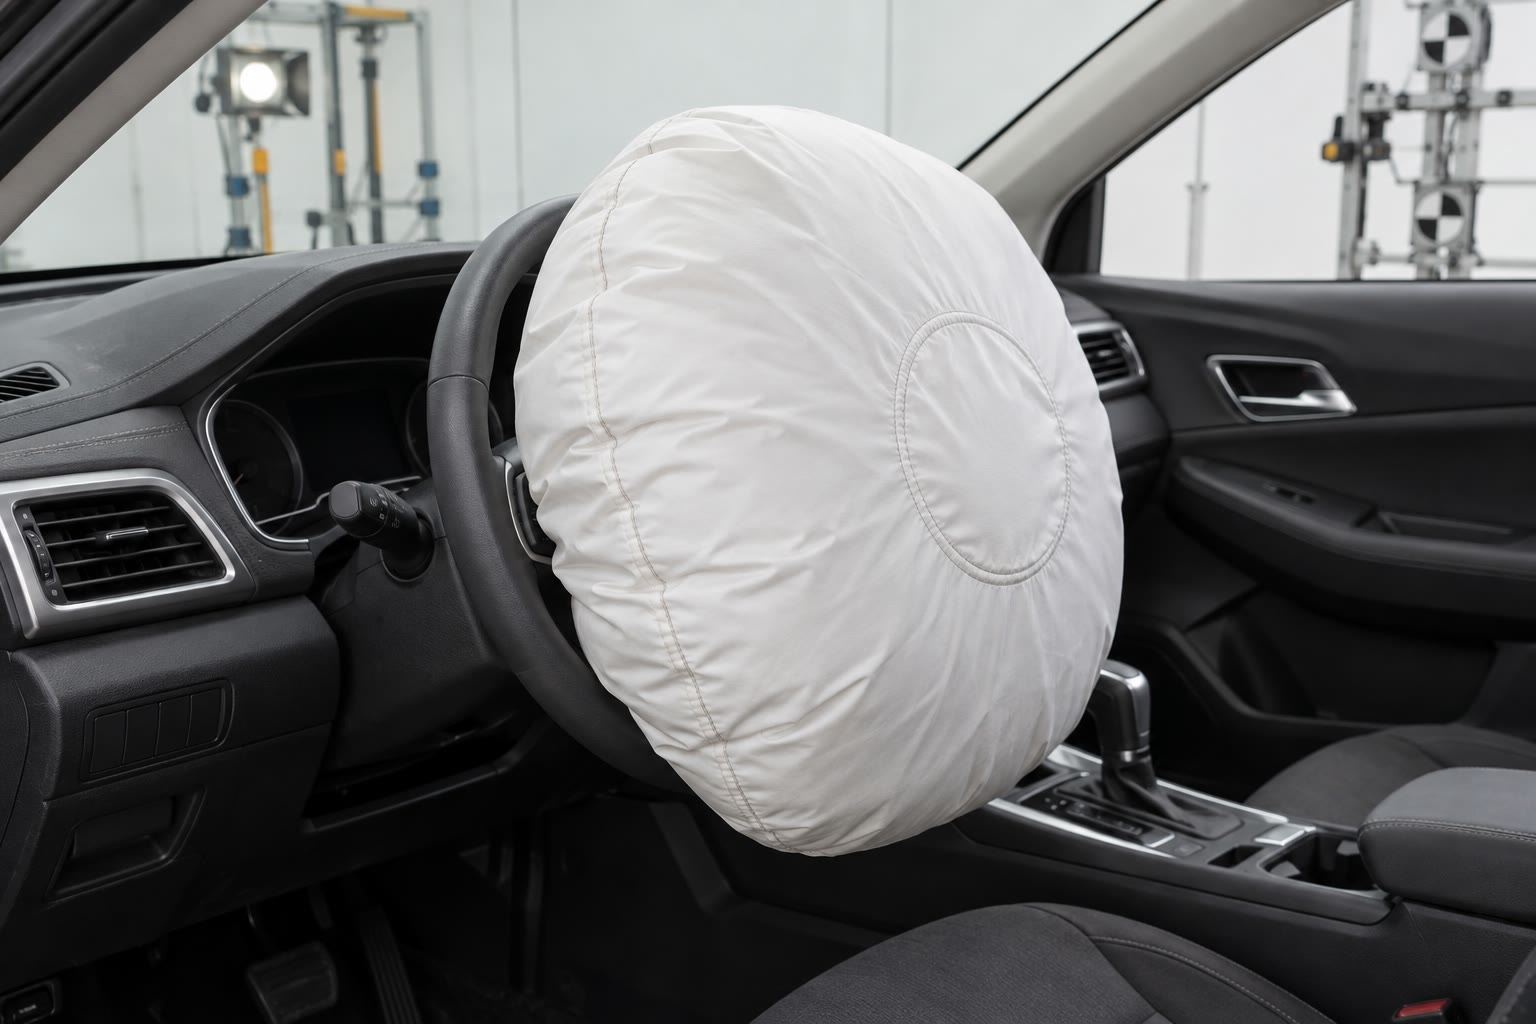
\includegraphics[width=0.5\linewidth]{images/book1/ai/g10-airbag.jpg}

{\small An airbag fills in a fraction of a second, with the nitrogen made
by a reaction.}
\end{omfigure}

\section{Describing a chemical system}

\begin{definition}[Chemical system, initial and final states]\label{def:g10:reaction-progress-table:system}
A \emph{chemical system}\index{chemical system} is the collection of
\omterm{def:g6:pure-substances-and-mixtures:species}{chemical species} present in a given place (a flask, a cushion, a cell),
each with its amount and its physical state. The system before the
reaction starts is the \emph{initial state}\index{initial state}; the
system once the reaction has stopped is the \emph{final
state}\index{final state}.
\end{definition}


\begin{example}[Methane burning in a closed vessel]\label{ex:g10:reaction-progress-table:methane}
A closed vessel contains \qty{2.0}{mol} of methane and \qty{3.0}{mol} of
dioxygen; a spark sets off the \omterm{def:g4:what-a-fire-needs:burning}{combustion}
\ce{CH4 + 2O2 -> CO2 + 2H2O}. In the \omterm{def:g10:reaction-progress-table:system}{initial state} the system holds
\qty{2.0}{mol} of \ce{CH4(g)}, \qty{3.0}{mol} of \ce{O2(g)} and no
products. What is in the \omterm{def:g10:reaction-progress-table:system}{final state}? The rest of the chapter answers.
\end{example}

\section{The extent of reaction and the progress table}

\begin{definition}[Extent of reaction, progress table]\label{def:g10:reaction-progress-table:extent}
The \emph{extent of reaction}\index{extent of reaction} $x$, in \omterm{def:g10:the-mole:amount}{moles},
counts how many times the reaction, as written in the \omterm{def:g8:balanced-equations:equation}{balanced
equation}, has taken place: when the extent is $x$, a species of
coefficient $\nu$ has been used up (\omterm{def:g7:chemical-reactions:reactant}{reactant}) or formed (product) in the
amount $\nu x$. The \emph{progress table}\index{progress table} gives,
under the equation, the amount of every species in the \omterm{def:g10:reaction-progress-table:system}{initial state},
at an extent $x$, and in the \omterm{def:g10:reaction-progress-table:system}{final state}.
\end{definition}

\begin{method}[Filling a progress table]\label{met:g10:reaction-progress-table:fill}
\begin{enumerate}
  \item Write the \omterm{def:g8:balanced-equations:equation}{balanced equation} in the first row.
  \item \omterm{def:g10:reaction-progress-table:system}{Initial state} ($x = 0$): write the initial amount of each
        species under it.
  \item Intermediate state (extent $x$): each \omterm{def:g7:chemical-reactions:reactant}{reactant} of coefficient
        $\nu$ becomes $n_0 - \nu x$, each product $n_0 + \nu x$.
  \item \omterm{def:g10:reaction-progress-table:system}{Final state}: find $x_{\max}$ (next section) and put it into the
        expressions of the intermediate row.
\end{enumerate}
\end{method}

\begin{omfigure}
\renewcommand{\arraystretch}{1.25}
\begin{tabular}{l|c|cccc}
\hline
equation & & \ce{CH4} & $+$ \ce{2O2} & $\longrightarrow$ \ce{CO2} & $+$ \ce{2H2O} \\
\hline
state & extent (\si{mol}) & \multicolumn{4}{c}{amounts (\si{mol})} \\
\hline
initial & $0$ & $2.0$ & $3.0$ & $0$ & $0$ \\
intermediate & $x$ & $2.0 - x$ & $3.0 - 2x$ & $x$ & $2x$ \\
final & $x_{\max} = 1.5$ & $0.5$ & $0$ & $1.5$ & $3.0$ \\
\hline
\end{tabular}\par\medskip

{\small The \omterm{def:g10:reaction-progress-table:extent}{progress table} of the methane \omterm{def:g4:what-a-fire-needs:burning}{combustion} of the example.
Each column follows one species; the coefficients 2 of \ce{O2} and of
\ce{H2O} become the $2x$.}
\end{omfigure}

\section{The limiting reactant and the final state}

\begin{definition}[Limiting reactant, maximum extent, total reaction]\label{def:g10:reaction-progress-table:limiting}
A reaction is a \emph{total reaction}\index{total reaction} if it stops
only when one of its \omterm{def:g7:chemical-reactions:reactant}{reactants} is used up. That \omterm{def:g7:chemical-reactions:reactant}{reactant} is the
\emph{limiting reactant}\index{limiting reactant}; the other \omterm{def:g7:chemical-reactions:reactant}{reactants}
are in excess. The extent at which the limiting \omterm{def:g7:chemical-reactions:reactant}{reactant} runs out is the
\emph{maximum extent}\index{maximum extent} $x_{\max}$; the \omterm{def:g10:reaction-progress-table:system}{final state}
of a total reaction is the state at $x = x_{\max}$.
\end{definition}

\begin{method}[Finding the limiting reactant]\label{met:g10:reaction-progress-table:limiting}
\begin{enumerate}
  \item For each \omterm{def:g7:chemical-reactions:reactant}{reactant}, solve $n_0 - \nu x = 0$: the \omterm{def:g7:chemical-reactions:reactant}{reactant} would
        run out at $x = n_0 / \nu$.
  \item The smallest of these values is $x_{\max}$; the \omterm{def:g7:chemical-reactions:reactant}{reactant} that
        gives it is the \omterm{def:g10:reaction-progress-table:limiting}{limiting reactant}.
  \item Put $x_{\max}$ into the intermediate row to get the \omterm{def:g10:reaction-progress-table:system}{final state};
        check that no amount is negative.
\end{enumerate}
\end{method}

\begin{example}[Back to the methane]\label{ex:g10:reaction-progress-table:methane-final}
Methane would run out at $x = 2.0/1 = \qty{2.0}{mol}$, dioxygen at
$x = 3.0/2 = \qty{1.5}{mol}$. The smaller is \qty{1.5}{mol}: dioxygen is
the \omterm{def:g10:reaction-progress-table:limiting}{limiting reactant} and $x_{\max} = \qty{1.5}{mol}$. The \omterm{def:g10:reaction-progress-table:system}{final state}
holds \qty{0.5}{mol} of methane left over, no dioxygen,
\qty{1.5}{mol} of carbon dioxide and \qty{3.0}{mol} of water.
\end{example}

\begin{omfigure}
\begin{tikzpicture}
\begin{axis}[width=0.78\linewidth, height=6.2cm, xmin=0, xmax=2.05,
    ymin=0, ymax=4.2, xlabel={extent $x$ (\si{mol})},
    ylabel={amount (\si{mol})}, axis lines*=left, ymajorgrids,
    grid style={gray!20}, tick label style={font=\small},
    label style={font=\small}, xtick={0,0.5,1,1.5,2},
    legend style={font=\small, at={(1.02,0.5)}, anchor=west, draw=none},
    legend cell align=left]
  \addplot[very thick, omDef, domain=0:2] {2-x};
  \addplot[very thick, omThm, domain=0:1.5] {3-2*x};
  \addplot[very thick, omMeth, domain=0:2] {x};
  \addplot[very thick, omProp, domain=0:2] {2*x};
  \legend{\ce{CH4}, \ce{O2}, \ce{CO2}, \ce{H2O}}
  \addplot[dashed, black!60] coordinates {(1.5,0) (1.5,4.2)};
  \node[font=\small, anchor=south west] at (axis cs:1.5,3.55) {$x_{\max}$};
  \fill[black!8, opacity=0.6] (axis cs:1.5,0) rectangle (axis cs:2.05,4.2);
\end{axis}
\end{tikzpicture}

{\small Amounts against the extent for the methane example. Dioxygen
(red) reaches zero first, at $x = \qty{1.5}{mol}$: the reaction stops
there, and the shaded part is never reached.}
\end{omfigure}

\begin{remark}[Not all reactions are total]\label{rem:g10:reaction-progress-table:not-total}
Many reactions stop before any \omterm{def:g7:chemical-reactions:reactant}{reactant} is used up: they reach a state
in which \omterm{def:g7:chemical-reactions:reactant}{reactants} and products coexist. Their \omterm{def:g10:reaction-progress-table:system}{final state} is not
$x_{\max}$, and a later chapter learns to find it. In this chapter, every
reaction is total.
\end{remark}

\section{The stoichiometric mixture}

\begin{definition}[Stoichiometric mixture]\label{def:g10:reaction-progress-table:stoichiometric}
A \omterm{def:g6:pure-substances-and-mixtures:mixture}{mixture} of \omterm{def:g7:chemical-reactions:reactant}{reactants} is a \emph{stoichiometric
mixture}\index{stoichiometric mixture} when the initial amounts are in
the proportions of the coefficients of the \omterm{def:g8:balanced-equations:equation}{balanced equation}.
\end{definition}

\begin{proposition}[All reactants run out together]\label{prop:g10:reaction-progress-table:together}
For a reaction $a\,\ce{A} + b\,\ce{B} \longrightarrow$ products, the \omterm{def:g6:pure-substances-and-mixtures:mixture}{mixture} is stoichiometric if
and only if
\[
  \frac{n_0(\ce{A})}{a} = \frac{n_0(\ce{B})}{b},
\]
and then, for a \omterm{def:g10:reaction-progress-table:limiting}{total reaction}, both \omterm{def:g7:chemical-reactions:reactant}{reactants} are used up in the \omterm{def:g10:reaction-progress-table:system}{final
state}.
\end{proposition}

\begin{proof}
\ce{A} would run out at $x = n_0(\ce{A})/a$, \ce{B} at $x = n_0(\ce{B})/b$.
The two values are equal exactly when the proportions are those of the
equation, and then the extent $x_{\max}$ empties both at once.
\end{proof}

\begin{example}[Burning methane cleanly]\label{ex:g10:reaction-progress-table:stoich}
For \ce{CH4 + 2O2 -> CO2 + 2H2O}, \qty{2.0}{mol} of methane need
\qty{4.0}{mol} of dioxygen: $2.0/1 = 4.0/2$. With only \qty{3.0}{mol}
of dioxygen the \omterm{def:g6:pure-substances-and-mixtures:mixture}{mixture} of the first example was short of oxygen; in a
real flame, that shortage is what makes the poisonous carbon monoxide
(\cref{ch:g8:combustion-and-fuels}).
\end{example}

\section{Gases and solutions in the table}


\begin{method}[Amounts for the initial state]\label{met:g10:reaction-progress-table:amounts}
Before filling a table, convert every quantity given into an amount:
$n = m/M$ for a solid or a liquid weighed; $n = V/V_m$ for a gas;
$n = c \times V$ for a dissolved species. At the end, convert back the
amounts of the \omterm{def:g10:reaction-progress-table:system}{final state} into whatever is asked: mass, gas volume or
concentration.
\end{method}

\begin{example}[Magnesium in hydrochloric acid]\label{ex:g10:reaction-progress-table:magnesium}
% ledger: aw:Mg
Hydrochloric acid contains hydrogen \omterm{def:g9:ions:ion}{ions} \ce{H+}, which attack magnesium:
\ce{Mg + 2H+ -> Mg^{2+} + H2}. A ribbon of \qty{0.12}{g} of magnesium is
dropped into \qty{50.0}{mL} of acid with $c(\ce{H+}) = \qty{1.0}{mol/L}$.
Initial amounts: $n_0(\ce{Mg}) = 0.12/24.3 = \qty{4.9e-3}{mol}$ and
$n_0(\ce{H+}) = 1.0 \times 0.0500 = \qty{5.0e-2}{mol}$. Magnesium would
run out at $x = \qty{4.9e-3}{mol}$, the hydrogen \omterm{def:g9:ions:ion}{ions} at
$x = 0.050/2 = \qty{2.5e-2}{mol}$: magnesium is limiting and
$x_{\max} = \qty{4.9e-3}{mol}$. The reaction gives \qty{4.9e-3}{mol} of
dihydrogen, that is $\num{4.9e-3} \times 24.1 = \qty{0.12}{L}$ at
\qty{20}{\celsius}, and leaves $0.050 - 2 \times 0.0049 =
\qty{0.040}{mol}$ of hydrogen \omterm{def:g9:ions:ion}{ions} in excess.
\end{example}

\begin{inthelab}[Balloons on flasks]
The teacher pours \qty{50.0}{mL} of the same hydrochloric acid into each
of six conical flasks, and places in six balloons increasing masses of
magnesium powder: 0.15, 0.30, 0.45, 0.60, 0.75 and \qty{0.90}{g}. Each
balloon is stretched over the neck of its flask, then lifted so that
the powder falls into the acid. Fizzing, the balloons swell. When all
has stopped, the balloons are larger and larger from the first flask to
the fourth; the fourth, fifth and sixth are the same size, and in the
last two some grey powder is left at the bottom of the flask.
\end{inthelab}

\begin{omfigure}
\begin{tikzpicture}[font=\small, scale=0.82]
  % H2 volume (L): 0.149 0.298 0.446 0.595 0.6025 0.6025; radius ~ V^(1/3)
  \foreach \i/\m/\v/\r/\left in {0/0.15/0.15/0.42/0, 1/0.30/0.30/0.53/0,
      2/0.45/0.45/0.61/0, 3/0.60/0.60/0.67/0, 4/0.75/0.60/0.67/1,
      5/0.90/0.60/0.67/1} {
    \begin{scope}[shift={(2.35*\i,0)}]
      \pic[transform shape] at (0,0) {erlenmeyer={0.25}{omWater}};
      \ifnum\left=1
        \fill[black!45] (-0.5,0.03) rectangle (0.5,0.12);
      \fi
      \fill[omProp!35, draw=omProp!80!black] (-0.3,2.6) -- (0.3,2.6)
        -- (0.12,2.82) -- (-0.12,2.82) -- cycle;
      \shade[ball color=omProp!40, draw=omProp!80!black]
        (0,{2.78+\r}) circle (\r);
      \node[align=center, anchor=north] at (0,-0.15)
        {\qty{\m}{g} Mg\\ \qty{\v}{L}};
    \end{scope}
  }
\end{tikzpicture}

{\small Six flasks with the same acid and growing masses of magnesium,
with the volume of dihydrogen (at \qty{20}{\celsius}) in each balloon.
Beyond about \qty{0.61}{g} the acid is limiting: the balloons stop
growing and magnesium is left over (grey).}
\end{omfigure}

\begin{remark}[Reading the plateau]\label{rem:g10:reaction-progress-table:plateau}
In the first flasks magnesium is the \omterm{def:g10:reaction-progress-table:limiting}{limiting reactant}, and doubling it
doubles the gas. From a certain mass on, the hydrogen \omterm{def:g9:ions:ion}{ions} run out
first: adding magnesium changes nothing but the leftover powder. The
change happens exactly at the \omterm{def:g10:reaction-progress-table:stoichiometric}{stoichiometric mixture},
$n_0(\ce{Mg}) = n_0(\ce{H+})/2 = \qty{0.025}{mol}$, that is
$0.025 \times 24.3 = \qty{0.61}{g}$ of magnesium.
\end{remark}

\begin{safety}{\ghs[0.82cm]{GHS02}\ghs[0.82cm]{GHS05}\ghs[0.82cm]{GHS07}}
% ledger: ghs:Mg, ghs:HCl
Magnesium powder is flammable; hydrochloric acid burns the skin and the
eyes and its fumes irritate the airways; dihydrogen burns in \omterm{def:g4:air-a-mixture-of-gases:air}{air}. A
demonstration by the teacher, with goggles, away from any flame.
\end{safety}

\section{Exercises}

\begin{exercise}[$\star$]\label{exo:g10:reaction-progress-table:1}
Fill the \omterm{def:g10:reaction-progress-table:extent}{progress table} of \ce{2H2 + O2 -> 2H2O} for an initial \omterm{def:g6:pure-substances-and-mixtures:mixture}{mixture}
of \qty{4.0}{mol} of dihydrogen and \qty{3.0}{mol} of dioxygen, assuming
the reaction is total. Give $x_{\max}$, the \omterm{def:g10:reaction-progress-table:limiting}{limiting reactant} and the
\omterm{def:g10:reaction-progress-table:system}{final state}.
\end{exercise}

\begin{exercise}[$\star$]\label{exo:g10:reaction-progress-table:2}
Carbon burns in dioxygen: \ce{C + O2 -> CO2}. Starting from \qty{3.0}{mol}
of carbon and \qty{2.0}{mol} of dioxygen, find $x_{\max}$, the \omterm{def:g10:reaction-progress-table:limiting}{limiting
reactant} and the \omterm{def:g10:reaction-progress-table:system}{final state}.
\end{exercise}

\begin{exercise}[$\star$]\label{exo:g10:reaction-progress-table:3}
Iron and sulfur react when heated: \ce{Fe + S -> FeS}. Starting from
\qty{0.50}{mol} of iron and \qty{0.30}{mol} of sulfur, describe the
\omterm{def:g10:reaction-progress-table:system}{final state}.
\end{exercise}

\begin{exercise}[$\star$]\label{exo:g10:reaction-progress-table:4}
Assume the reaction \ce{N2 + 3H2 -> 2NH3} is total. Starting from
\qty{1.0}{mol} of dinitrogen and \qty{2.4}{mol} of dihydrogen, find
$x_{\max}$ and the \omterm{def:g10:reaction-progress-table:system}{final state}.
\end{exercise}

\begin{exercise}[$\star$]\label{exo:g10:reaction-progress-table:5}
For \ce{2CO + O2 -> 2CO2}, which of these \omterm{def:g6:pure-substances-and-mixtures:mixture}{mixtures} is stoichiometric?
(a) \qty{2}{mol} \ce{CO} and \qty{2}{mol} \ce{O2}; (b) \qty{4}{mol}
\ce{CO} and \qty{2}{mol} \ce{O2}; (c) \qty{1}{mol} \ce{CO} and
\qty{2}{mol} \ce{O2}.
\end{exercise}

\begin{exercise}[$\star\star$]\label{exo:g10:reaction-progress-table:6}
What mass of dioxygen is needed to burn \qty{32}{g} of methane completely
(\ce{CH4 + 2O2 -> CO2 + 2H2O})? What mass of water is formed?
\end{exercise}

\begin{exercise}[$\star\star$]\label{exo:g10:reaction-progress-table:7}
A camping stove burns \qty{1.0}{kg} of propane:
\ce{C3H8 + 5O2 -> 3CO2 + 4H2O}. What volume of carbon dioxide, at
\qty{20}{\celsius}, does it release?
\end{exercise}

\begin{exercise}[$\star\star$]\label{exo:g10:reaction-progress-table:8}
Using the figure of the amounts against the extent for the methane
example, read the amounts of the four species at $x = \qty{1.0}{mol}$.
Why does the line of dioxygen stop at $x = \qty{1.5}{mol}$?
\end{exercise}

\begin{exercise}[$\star\star$]\label{exo:g10:reaction-progress-table:9}
\qty{1.30}{g} of zinc powder are added to \qty{100.0}{mL} of blue copper
sulfate solution at \qty{0.10}{mol/L}. The reaction is
\ce{Zn + Cu^{2+} -> Zn^{2+} + Cu}.
Find the \omterm{def:g10:reaction-progress-table:limiting}{limiting reactant}, the mass of copper formed and the mass of
zinc left. Is the solution still blue at the end?
\end{exercise}

\begin{exercise}[$\star\star$]\label{exo:g10:reaction-progress-table:10}
\qty{0.48}{g} of magnesium are added to \qty{20.0}{mL} of hydrochloric
acid with $c(\ce{H+}) = \qty{1.0}{mol/L}$
(\ce{Mg + 2H+ -> Mg^{2+} + H2}). Which \omterm{def:g7:chemical-reactions:reactant}{reactant} is limiting? What volume
of dihydrogen is collected at \qty{20}{\celsius}?
\end{exercise}

\begin{exercise}[$\star\star$]\label{exo:g10:reaction-progress-table:11}
In exercise~3, by what percentage is the \omterm{def:g7:chemical-reactions:reactant}{reactant} in excess above the
amount that would have made a \omterm{def:g10:reaction-progress-table:stoichiometric}{stoichiometric mixture}?
\end{exercise}

\begin{exercise}[$\star\star\star$]\label{exo:g10:reaction-progress-table:12}
A student wants \qty{10.0}{g} of a \omterm{def:g10:reaction-progress-table:stoichiometric}{stoichiometric mixture} of iron and
sulfur for \ce{Fe + S -> FeS}. What masses of iron and of sulfur must be
weighed?
\end{exercise}

\begin{exercise}[$\star\star\star$]\label{exo:g10:reaction-progress-table:13}
\qty{10.0}{g} of limestone \ce{CaCO3} are strongly heated and decompose
totally: \ce{CaCO3 -> CaO + CO2}. The quicklime \ce{CaO} obtained is then
put into \qty{1.8}{g} of water: \ce{CaO + H2O -> Ca(OH)2}.
\begin{enumerate}
  \item Fill the \omterm{def:g10:reaction-progress-table:extent}{progress table} of the first reaction; what volume of
        carbon dioxide is released at \qty{20}{\celsius}?
  \item Fill the table of the second reaction. Which \omterm{def:g7:chemical-reactions:reactant}{reactant} is
        limiting? What mass of slaked lime \ce{Ca(OH)2} is formed?
\end{enumerate}
\end{exercise}

\begin{exercise}[$\star\star\star$]\label{exo:g10:reaction-progress-table:14}
In the balloon experiment of the lab box, compute the volume of
dihydrogen in each balloon. Explain why it stops growing after the
fourth flask, and plot (by hand) the volume of gas against the mass of
magnesium.
\end{exercise}

\begin{exercise}[$\star\star\star$]\label{exo:g10:reaction-progress-table:15}
\qty{4.6}{g} of ethanol \ce{C2H6O} burn in a closed vessel containing
\qty{4.8}{L} of dioxygen at \qty{20}{\celsius}:
\ce{C2H6O + 3O2 -> 2CO2 + 3H2O}. Find the \omterm{def:g10:reaction-progress-table:limiting}{limiting reactant}, the mass of
ethanol left unburnt and the volume of carbon dioxide formed.
\end{exercise}

\section{Problem: The Airbag}

\begin{problem}[{Weekend problem --- what mass of sodium azide must be
packed into a steering wheel to fill a 60-litre airbag?}]
\label{pb:g10:reaction-progress-table:1}
% ledger: use:NaN3-airbag, ghs:NaN3, aw:Na, aw:N, aw:K, aw:O
In the classic airbag design, an electric spark sets off the
decomposition of solid sodium azide:
\[
  \ce{2NaN3 -> 2Na + 3N2} .
\]
The sodium \omterm{def:g9:periodic-table-first-look:metal}{metal} formed is dangerous: it reacts violently with water,
and with the moisture of the skin and the eyes. The charge therefore
also contains potassium nitrate, which turns the sodium into harmless
oxides and gives a little more nitrogen:
\[
  \ce{10Na + 2KNO3 -> K2O + 5Na2O + N2} .
\]
Both reactions are total. The airbag must be filled with \qty{60}{L} of
nitrogen; take the gas at \qty{20}{\celsius}, where
$V_m = \qty{24.1}{L/mol}$.

\medskip
\noindent\textbf{Part I --- The reactions.}
\begin{enumerate}
  \item Check that the first equation is balanced, element by element.
  \item Check that the second equation is balanced.
  \item Which earlier chapter showed that sodium reacts violently with
        water? Why must no sodium remain after the crash?
  \item Compute the molar masses of sodium azide \ce{NaN3} and of
        potassium nitrate \ce{KNO3}.
\end{enumerate}

\medskip
\noindent\textbf{Part II --- The decomposition.}
\begin{enumerate}[resume]
  \item Fill the \omterm{def:g10:reaction-progress-table:extent}{progress table} of the first reaction for an initial
        amount of \qty{1.00}{mol} of sodium azide.
  \item Find $x_{\max}$. Which is the \omterm{def:g10:reaction-progress-table:limiting}{limiting reactant}?
  \item Give the amounts of sodium and of nitrogen in the \omterm{def:g10:reaction-progress-table:system}{final state}.
  \item What volume of nitrogen does \qty{1.00}{mol} of sodium azide give
        at \qty{20}{\celsius}?
\end{enumerate}

\medskip
\noindent\textbf{Part III --- Removing the sodium.}
\begin{enumerate}[resume]
  \item Fill the \omterm{def:g10:reaction-progress-table:extent}{progress table} of the second reaction, starting from
        the sodium found in question 7 and an amount $n$ of potassium
        nitrate.
  \item What amount, and what mass, of potassium nitrate makes a
        \omterm{def:g10:reaction-progress-table:stoichiometric}{stoichiometric mixture} with this sodium?
  \item Give the \omterm{def:g10:reaction-progress-table:system}{final state} of the second reaction for this \omterm{def:g6:pure-substances-and-mixtures:mixture}{mixture}.
  \item If only \qty{0.150}{mol} of potassium nitrate were put in, which
        \omterm{def:g7:chemical-reactions:reactant}{reactant} would be limiting, and what would be left? Why would
        that be dangerous?
\end{enumerate}

\medskip
\noindent\textbf{Part IV --- The 60-litre bag.}
\begin{enumerate}[resume]
  \item From questions 7 and 11, what amount of nitrogen does the whole
        charge give per \omterm{def:g10:the-mole:amount}{mole} of sodium azide?
  \item What amount of nitrogen fills the bag?
  \item Deduce the amount of sodium azide needed.
  \item Compute its mass.
  \item Compute the mass of potassium nitrate to add.
  \item Without the second reaction, what mass of sodium azide would
        have been needed? How much does the second reaction save?
  \item Sodium azide is fatal if swallowed. Why does it matter that the
        first reaction is total, and how does the \omterm{def:g10:reaction-progress-table:extent}{progress table} show
        that none is left?
  \item State the final answer: what mass of sodium azide fills a
        \qty{60}{L} airbag?
\end{enumerate}
\end{problem}
